
\chapter{Engineering Deconstruction}
\label{chp:engineering}

Given the design challenge of creating a simulation assisted visual
system for authoring plastic surgery procedures, the next problem is
determining by what methods can we best accomplish this
task. Commercially, there exist examples of surgical simulation
products based on both procedural animations and physical
simulations. As discussed in the previous chapter, a detailed
procedural animation can accommodate some, but not all, of the goals
for a surgical authoring system. Procedural animation methods can
provide realistic geometry, respond to user inputs by advancing down
pre-scripted event chains, and serve as a functional replacement for
traditional illustrated procedure guides. However, procedural approaches
fall short when assisting in cognitive training tasks.

Under cognitive training, the surgeon is expected to be developing a
mental intuition for how operations work at a fundamental level and be
capable of adapting this knowledge to new situations. These
requirements go beyond a simple recall of a ``correct'' approach, but
to understand why these techniques work as they do. Traditionally,
this level of understanding is gained through years of experience
working with live patients or animal models. Through this process,
surgeons experiment with designs (guided by experienced mentors) and
observe the results in order to better understand what works and what
does not. Supporting this style of intellectual freedom, the
ability to deviate from diagrams in textbooks, is the goal of the
plastic surgery simulation system we wish to build. To address these
concerns, we turn away from procedural animations to physical
simulation. Physical simulation can address this problem by
providing correct, real-time responses to a user's actions, instead of
forcing them into pre-scripted routines.

The remaining chapters in this document will discuss technical
contributions that form the foundation of the plastic surgery
benchmark application described in the previous chapter. The goal of
this chapter is to deconstruct the basic engineering challenges found
in this space. This deconstruction will frame the work presented in
subsequent chapters, which can otherwise feel somewhat disconnected
from the topic of plastic surgery.

\section{Background}

To start, let us bring the topic of discussion down from the general
specifications discussed in the previous chapter and provide a
concrete goal for what we want to provide. At the core, our proposed
surgical application can be described as a system which instills a
reactive mechanical response into three dimensional models of tissue
to static and animated constraints. Let us break this goal down
further and look at each of these parts in more detail.

To begin, let us start with the concept of mechanical
response. Mechanical response of soft bodies, such as human tissue,
can be described as a series of relationships between shape, forces,
and energy. At a very high level, when forces act on an object and
alter its shape, this requires a proportional amount of energy, which
is then stored by the object. In real materials, this potential energy can be
dissipated in many ways, such as heat or \textit{by further changes in
shape}. Our goal in the simulation of elastic materials is to minimize
the energy of our virtual materials by this latter outcome. In other
words, we attempt to compute new shapes, which minimize the energy of
the object, in response to external conditions and forces. The precise
form of these shapes depends on the material of the object. For our
purposes, we are interested in a family of materials known as
\textit{hyperelastic} materials. The energy of these materials depends
only on the object's current shape and do not consider the history of
the object's shape, only its initial and final ones. While these
materials are idealized, they are most similar to rubbers or other
materials that ``bounce back'' after being deformed.

If mechanical response is the relationship between shape, energy, and
forces, shape itself is the physical extents of the object. If we
consider the virtual tissue models we are interested in simulating,
they can be described geometrically as a closed boundary in a three
dimensional coordinate system and the region the boundary encloses,
which we represent by $\Omega$. For the moment we will consider this
domain to be a continuous volume. In a later section, we will discuss
how this domain can be stored discretely on a computer.

The last part, relating to constraints, we will hold off on for now. We
will return to this idea at the end of the chapter, once we have
covered the mathematical and computational details surrounding
mechanical response and shape, which will be the topic of the next two
sections.


% First, what does it mean to have a three dimensional tissue model with
% mechanical responses?  Starting from the real world, tissues are
% fundamentally collections of cells, or more basically,
% atoms. Considering the collection as a whole, these small elements
% give rise to the tissue's shape and form. We will return to this idea
% of small elements later in the chapter, but for now let us pretend
% that these materials are continuous entities. We do this
% for the convenience of reasoning about them in a mathematical sense,
% for ultimately all of the complex physical behaviors we expect from
% soft, squishy materials can be described by equations for stress and
% strain.

% To begin, we can consider an abstraction: a model of
% tissue which consists of a closed boundary in three dimensional
% coordinate system and the region which it encloses. We will be
% referring to this region of space as the object's domain, represented
% by the symbol $\Omega$. Later, we will talk about how to represent
% this domain discretely on a computer, but for now simply treat it as a
% prescribed region.

% The next challenge is to describe what we mean by mechanical
% response. Mechanical response of soft bodies, such as human tissue,
% can be described as a series of relationships between shape, forces,
% and energy. We will be using these relationships to convert between
% one aspect and another - in other words, produce new shapes from
% considering the forces applied to an object. To explain this idea, let
% us first consider a hypothetical elastic object, such as a block of
% rubber. If one was to squeeze the block from two opposite sides, it
% would deform, or change shape. And if the block is released, the shape
% returns to the original configuration. What is happening in this
% situation is the physical manifestation of the relationship between
% the applied forces, the block's internal energy, and its shape. In
% particular, we are primarily interested in a class of materials known
% as hyperelastic materials. These materials are idealized as they do
% not consider the object's prior deformation history when we compute
% their internal energy, depending only on the current shape of the
% object. The alternative would be some degree of plasticity, where
% deformation imparts some long lasting effect on the material. Plastic
% effects are incredibly common in real life, from the persistent
% wrinkles in uncrumpled paper to the fact that metal holds its shape
% after being bent. We can avoid introducing the complexity of these
% effects by noting that human tissue, which does exhibit plastic effects
% over long periods of time, is effectively hyperelastic during the time
% frame of a typical surgical operation. In the next section, we'll see
% how to define this relationship between shape, force, and energy more
% mathematically.


\section{Continuous Formulation of Deformation}




In this section, we will expand on the relationship between shape,
energy, and force from the previous section and provide a mathematical
foundation which we will later use for discrete computations. The
first idea we need to explore is that of shape change itself. When an
object changes shape from one configuration to another, we refer to
this as a \textit{deformation}. To keep track of the deformation, we
record it relative to the object's reference configuration. This is an arbitrarily
chosen shape in the coordinate system of the object from which all
other deformations are measured. Mathematically, we can define the deformation as
a mapping between the locations in the domain of the object and $\mathbf{R}^3$:
\begin{equation}
  \phi: \Omega \subset \mathbf{R}^3 \rightarrow \mathbf{R}^3
\end{equation}
Under this regime, we consider the domain of $\phi$ to be points in
$\Omega$, often referred to as material space locations as they can
conceptually be considered infinitesimal blobs of undeformed
material. We simultaneously locate and identify them by a spatial
vector: $\vec{X} = (X, Y, Z)$. The points in $R^3$ which make up the
image of $\phi$ are the corresponding deformed locations
$\vec{x} = (x, y, z)$. This relationship can be seen in Figure
\ref{fig:deformationexample}.


\begin{figure}[t]
  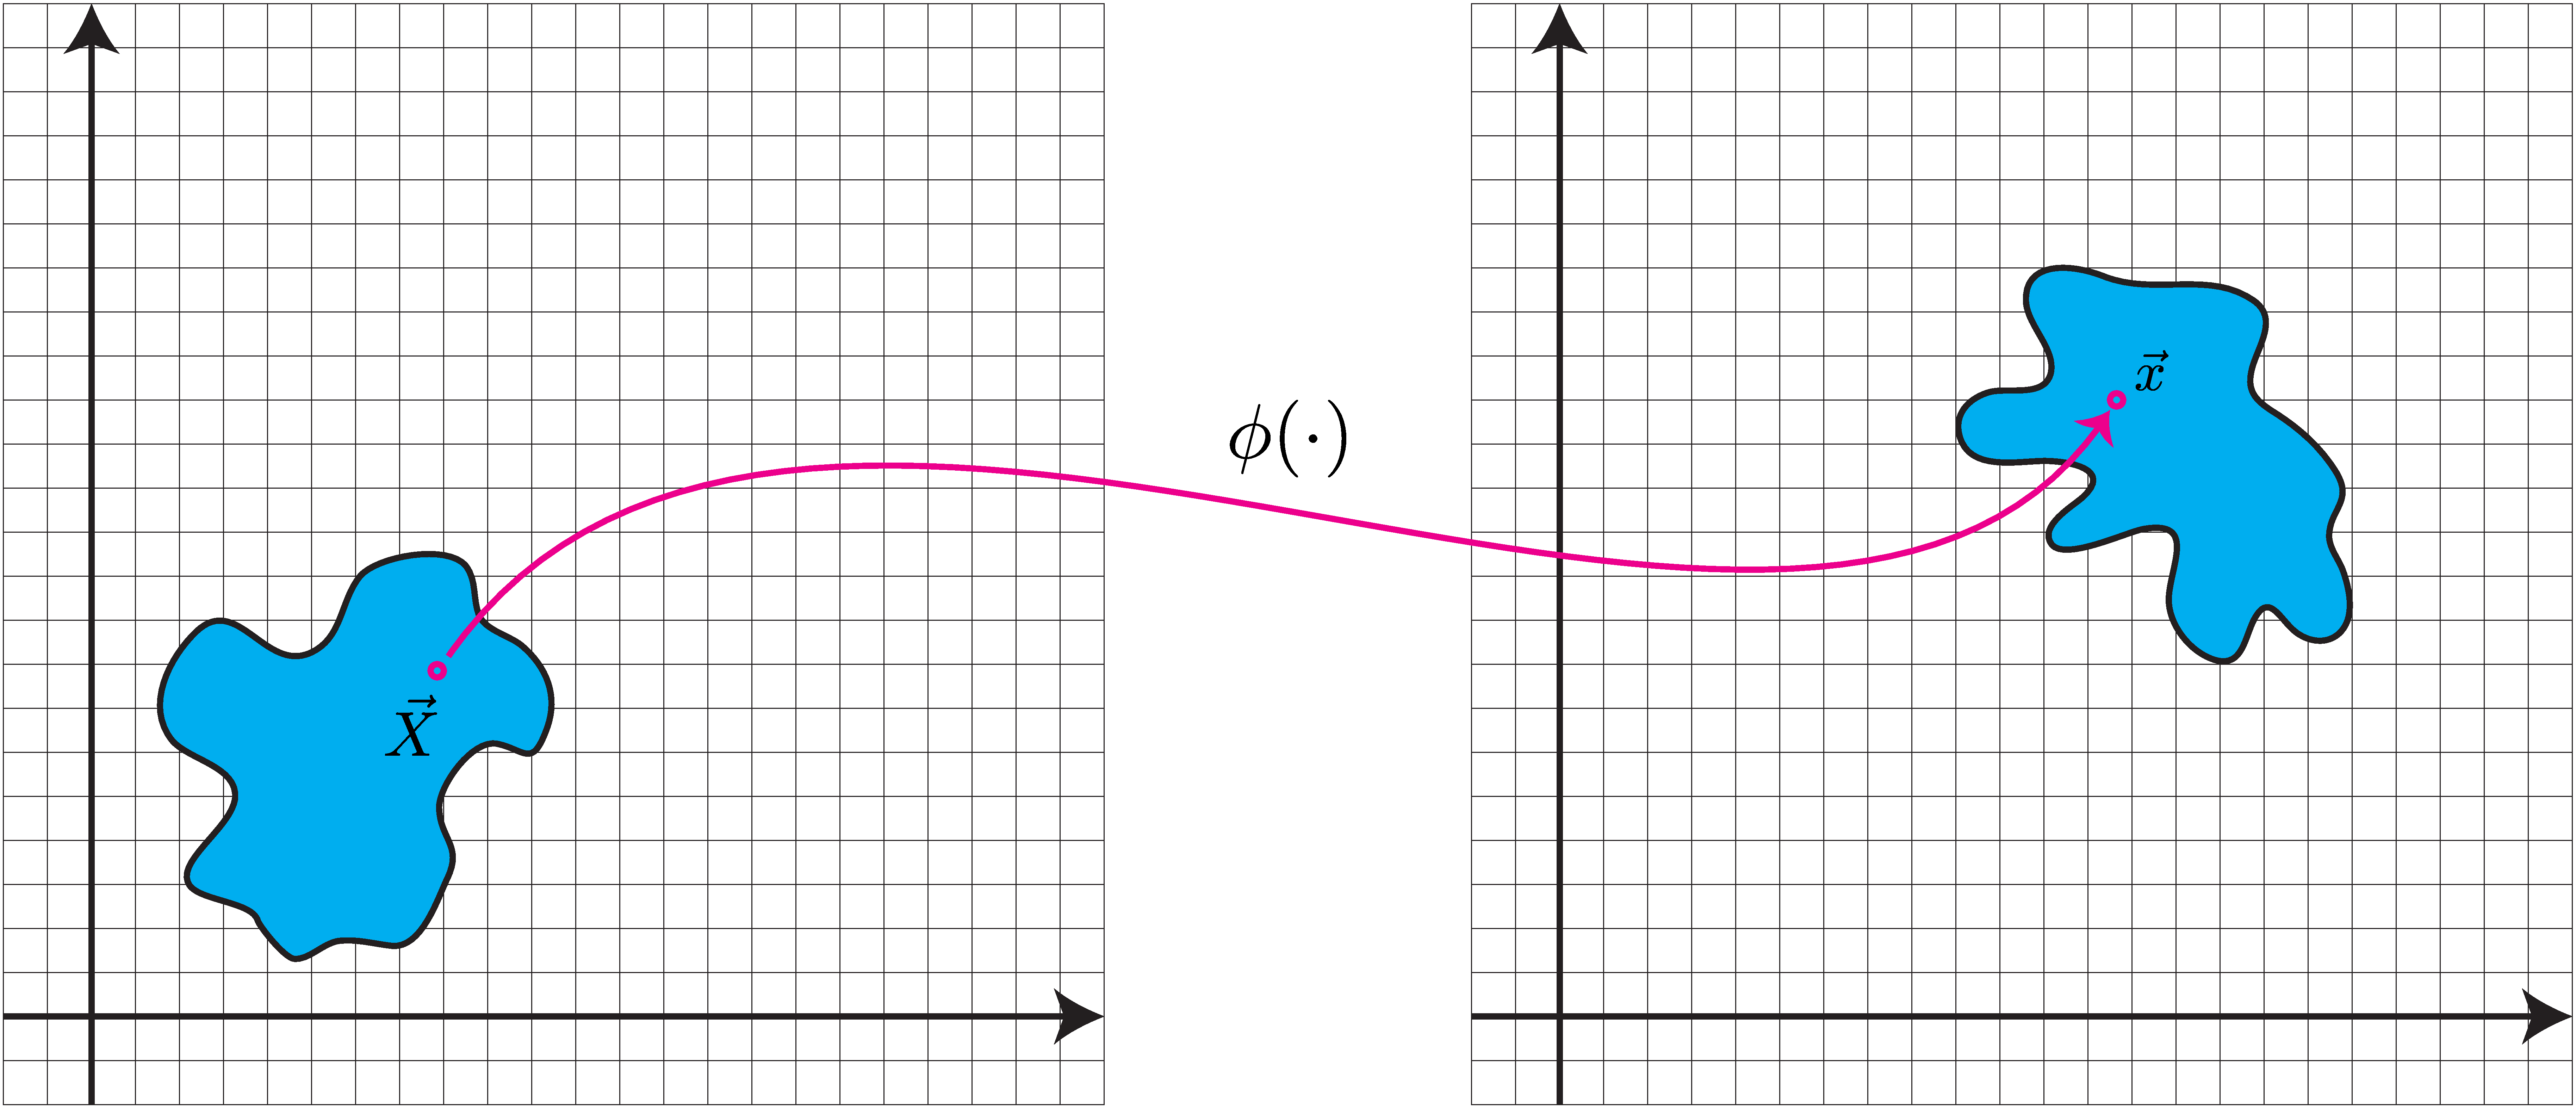
\includegraphics[width=\textwidth]{other_images/DeformationFigure.pdf}
  \vspace*{-.3in}
   \caption{Example Deformation Map}{The deformation map $\phi$ is
     illustrated here mapping between locations $\vec{X}$ in the
     object's reference configuration and corresponding deformed
     locations $\vec{x}$ in the object's deformed configuration.}
   \label{fig:deformationexample}
   \vspace*{-.15in}
\end{figure}

% If we recall Newton's Third Law of Motion, external forces applied to
% objects are met with an equal and opposite force. But if we look at
% the object fractionally, we would see that these opposing forces
% don't just exist on the surface, but are distributed internally
% throughout the object's material. These internal forces are referred
% to as mechanical stress. Stress is defined to be force applied over an
% cross-sectional area, or volume for three dimensional objects. If we
% were to look at a single point of an object, we could define the
% internal stress of that point by a second dimensional tensor, which
% describes what force vectors are felt by that point in three
% orthogonal directions. Ultimately, this internal stress field causes
% the object to deform, or change shape, resulting in strain - the
% mechanical term for a related tensor value which is defined as the
% ratio of changed length (or volume) compared to the original
% length (or volume). The strain tensor, in combination with the specific material
% being deformed, represents a quantity of potential energy. This energy
% represents the amount of work required to deform the object.  Given
% these basic mechanical deformation concepts, we can now develop a
% theoretical framework for simulating deformable objects.

% The first part of that process is describing our representation of
% state. To do so, we return to the object's shape. The deformation of
% an object is the change in shape between one configuration and
% another. In order to keep track of the deformation, we can record it
% relative to an object's reference configuration. This is an arbitrarily
% chosen shape in the coordinate system of the object from which all
% other deformations are measured. Mathematically, we can define the deformation as
% a mapping between the locations in the domain of the object and $\mathbf{R}^3$:
% $$\phi: \Omega \rightarrow \mathbf{R}^3$$. Under this regime, we
% consider the domain of $\phi$ to be points in $\Omega$, often referred
% to as material space locations as they can conceptually be considered
% infinitesimal blobs of undeformed material. We simultaneously locate and
% identify them by a spatial vector: $\vec{X} = (X, Y, Z)$. The points
% in $R^3$ which make up the image of $\phi$ are the corresponding
% deformed locations $\vec{x} = (x, y, z)$. It is worth noting that the reverse mapping
% could have been considered, i.e the mapping that projects from a shape
% back to the reference configuration. This type of relationship is
% not unusual in computer graphics, for instance via mesh
% parameterization for texture mapping. Unfortunately, this relationship
% is a little harder to deal with, especially if we wish to handle
% situations where the mapping is not one-to-one, such as when the
% deformation causes the object to overlap with itself. For the
% techniques presented in this document, we will be using a reference
% configuration that avoids self penetration and a forward deformation
% map to avoid these problems.

Now that we have defined for what it means for an object to be
deformed and the concept of a deformation map, we can return to the
relationship between shape, force, and energy. In order to relate
shape, or deformation, of an object to its energy, we need to define a
way to measure how the deformation varies throughout the object. We
facilitate this by defining the quantity called the deformation
gradient $\mathbf F$, the jacobian of the deformation map.

\begin{equation}
  \label{equ:deformationgradient}
  \mathbf{F}(\vec{X}) = \frac{\partial \phi(
      \vec{X} )}{ \vec{X} }
\end{equation}

From the deformation gradient, we can extract metrics of deformation,
known as strain measures. The strain measure is directly used to
compute the strain energy, the potential energy of the material due to
deformation. In the reference configuration, we want the
strain measure to be evaluate to zero. Additionally, if the object's
deformation is purely translational, we would also like the strain
measure to be zero. A simple strain measure that meets these goals
might be:

\begin{equation}
  \label{equ:simplestrainmeasure}
  s = \mathbf F - \mathbf I
\end{equation}

While this evaluates to zero under translation and no deformation,
this simple measure is non-zero under rotation, which can result in
inaccuracies under large deformation. We can treat this issue by
employing a different strain measure, the Green strain $\mathbf{E}$:

\begin{equation}
  \label{equ:greenstrain}
  \mathbf{E} = \frac 1 2 (\mathbf{F}^T\mathbf{F}-\mathbf{I})
\end{equation}

The Green strain is more robust to large deformations by virtue of it
being rotation invariant, but is non-linear and can behave
non-intuitively around extreme deformations. As an example, consider a
deformation that simply inverts an object along one axis. The Green
strain of this deformation would be zero in this case despite a
significant deformation. If we take a linear approximation around the
undeformed configuration of the Green strain, we arrive at the
\textit{small strain} $\epsilon$:

\begin{equation}
  \label{equ:smallstrain}
  \bm{\epsilon} = \frac 1 2 (\mathbf{F} + \mathbf{F}^T) - \mathbf{I}
\end{equation}

This formula is linear and under small deformations is approximate to
the Green strain, making it useful for scenarios with limited
deformation, such as structural simulations for buildings or other
near rigid objects. As the deformation increases however, the small
strain suffers from the similar problems as the simple strain
presented earlier (Equation \ref{equ:simplestrainmeasure}).  In order to get a strain measure that is
rotationally invariant and is more predictable than the Green strain,
one possibility is to apply a polar decomposition to the deformation
gradient in order to extract the rotational components:
\begin{equation}
  \label{equ:polarstrain}
  \begin{split}
    \mathbf F &= \mathbf R\mathbf S\\
    \bm \epsilon_c &= \mathbf S - \mathbf I
  \end{split}
\end{equation}
While this strain measure is still non-linear, it behaves similarly to
the small strain measure, including a linear (not quadratic)
relationship to axis aligned stretch, while maintaining rotational
invariance.

Once we have chosen our strain measure, we can use it to define a
strain energy density $\Psi(\mathbf{F})$. This is a measure of the
potential energy per unit volume of the material as a consequence of
undergoing deformation.  Similar to the strain measure, there are
several popular energy density functions which can describe generic
deformable materials. Linear elasticity (Equation
\ref{equ:linearelasticity}), derived from the small strain tensor, is
easy and uncomplicated to compute due to its linear relationship to
the deformation gradient. However, since it is based on the small
strain tensor, it is not rotationally invariant and can exhibit
physically inaccurate behaviors under large deformations.

\begin{equation}
  \label{equ:linearelasticity}
  \Psi(\mathbf{F}) = \mu \bm \epsilon : \bm \epsilon + \frac \lambda 2
  \text{tr}^2(\bm \epsilon)
\end{equation}

If we replace the strain measure used in the Linear
elasticity model with the Green strain, we get what is known as
the St. Venant-Kirchhoff energy density function (Equation
\ref{equ:stvenantkirchhoff}).
\begin{equation}
  \label{equ:stvenantkirchhoff}
  \Psi(\mathbf{F}) = \mu \mathbf{E} : \mathbf{E} + \frac \lambda 2
  \text{tr}^2(\mathbf E)
\end{equation}
While this model is more accurate under large deformations due to the
Green strain, it has the unfortunate property of not penalizing
significant compression and inversion. In the film production
industry, another nonlinear energy function is often used instead,
called Co-rotated elasticity, which is based off the fourth strain
measure detailed in Equation \ref{equ:polarstrain}:

\begin{equation}
  \label{equ:corotatedelasticity}
  \begin{split}
   \Psi(\mathbf{F}) &= \mu \bm \epsilon_c : \bm \epsilon_c + \frac \lambda 2
   \text{tr}^2(\epsilon_c)\\ &= \mu \lVert \bm S - \bm I \rVert^2_{\bm
     F} + \frac \lambda 2
   \text{tr}^2(S-I)
   \end{split}
\end{equation}

Finally, we can calculate the energy of the entire object by
integrating the energy density over the domain:

\begin{equation}
  \label{equ:systemenergy}
  E(\phi) = \int_\Omega \Psi( \mathbf F ) \,d\vec{X}
\end{equation}

In the next section, we will convert these continuous equations of
deformation and energy into discrete forms, allowing us to solve for
our object's deformations. Up until now, the equations we have been
using have assumed a continuous deformation field, free of any
particular discretization. The expressions in the next section will
replace these continuous equations with those appropriate for the
lattice based discretization we use in our application.

\section{Discrete form of Elastic Deformation}
\label{sec:engineering:solving}

With these equations in hand, we can now reason about how to produce
realistic mechanical responses from our virtual tissue models on a
computer. To do so, we need to change how we have been treating the
expressions from the previous section from a continuous representation
to a discrete representation suitable for computation. To do this, we
will be dividing our continuous domain in to smaller regions, or
elements. Each element represents a finite quanta of material, thus
giving rise to the name of the approach we will be using throughout
this document: Finite Element Method (FEM).

In our new discrete world, we must first translate our former
continuous domain $\Omega$ into a data structure representable on a
computer. Here we have a number of choices to pick from. FEM
literature has described many approaches for discretization over the
years, ranging from volumetric meshes to particle based
approaches. These designs can be evaluated over several categories:
regularity, conformity, and ease of use. Regularity refers to the
extent that the technique uses repeating data structures or provides
implicit internal relationships that can be predicted, which is often
extremely beneficial for performance optimization. Conformity refers
to how the data structure represents the object's boundary shape,
either attempting to directly replicate the object's domain or acting
as a scaffolding around it, which can affect the accuracy of the
simulation. Finally, ease of use is a catch all term that includes any
property which makes the data structure easy or troublesome to include
in higher level pipelines. In this document, the approach we will be
using is a mesh discretization. In particular, we will be using a
design referred to as an embedding lattice. Seen in Figure
\ref{fig:embeddingexample}, we have an example mesh of a lion and its embedding lattice. This data structure is extremely regular
and generally easy to construct, though it can suffer from a lack of
conformity.

\begin{figure}[t]
  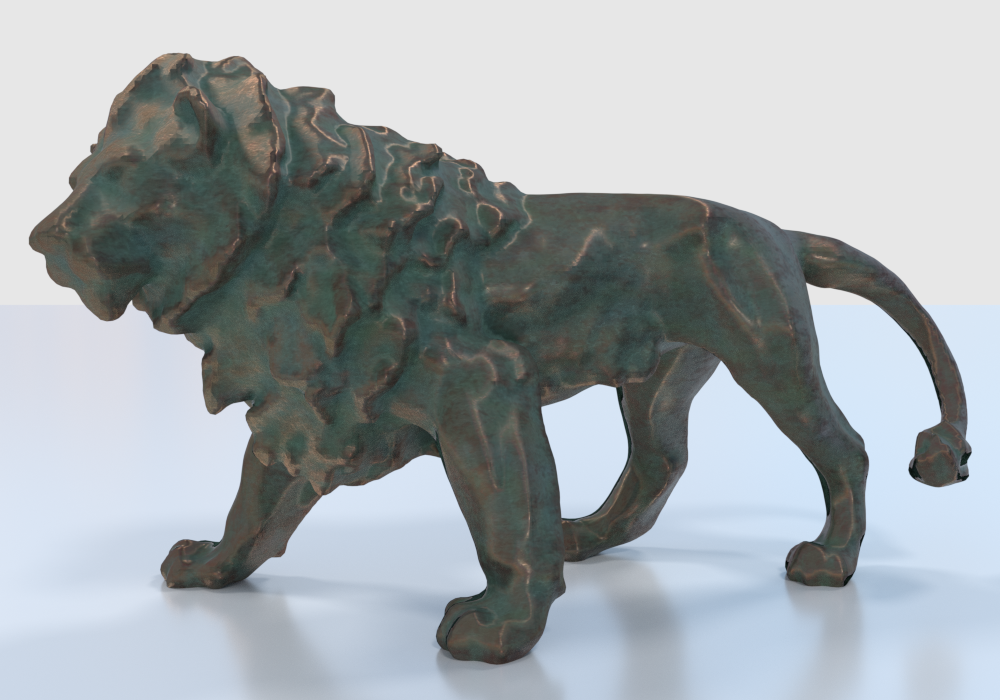
\includegraphics[width=.5\textwidth]{other_images/LionStatue.png}
  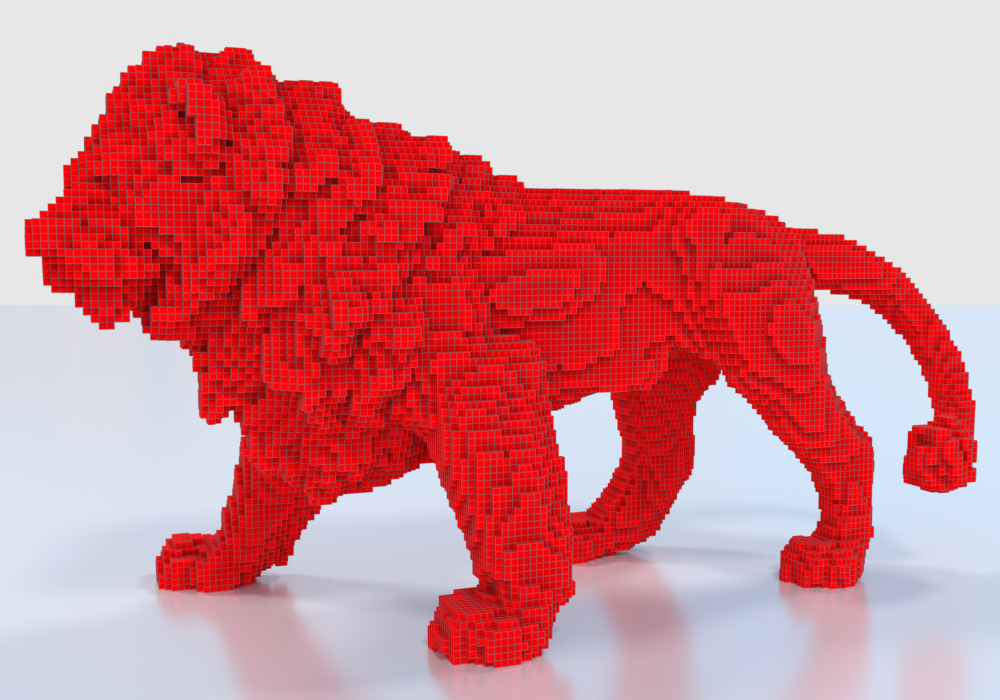
\includegraphics[width=.5\textwidth]{other_images/LionLattice.png}
  \vspace*{-.3in}
   \caption{Lattice Embedding}{Show here is a three dimensional lion
     model\footnotemark (left) and the corresponding embedding lattice
     (right). Each vertex of the lion model is embedded into a cell of
   the lattice, which acts as a deformable scaffold around the model.}
   \label{fig:embeddingexample}
   \vspace*{-.15in}
\end{figure}

\footnotetext{The lion model was rendered with a shader created
  by Anthony Pilon.}

Under this representation, our material will be sampled at Cartesian
\textit{nodes} of a regular hexahedral lattice and our elements of computation
will be its \textit{cells}. We refer to these nodes as containing degrees of freedom, as
they represent the discrete points where deformation can occur. To
deal with the issue of conformity, we utilize a technique known as
lattice embedding - whereby the discrete boundary of our object,
represented by a separate surface mesh, is embedded in cells of the lattice
via a weighted interpolation of its nodes. Later in this document,
additional techniques will be presented to further increase the
accuracy of the lattice's boundary conformity. Since the
terms presented in regards to embedding can be confusing, we will
stick to the following terminology:

\begin{description}
\item[lattice] - The simulation lattice is the discrete representation
  of our simulation domain and is composed of elements of material known
  as cells. Through the simulation lattice, we compute deformation
  gradients, energy, and ultimately forces.
\item[node] - A node is a topological point in our simulation
  lattice. Each node is identified by a spatial location as a label
  and stores three degrees of freedom, or DOFs. These degrees of
  freedom are represented by the discrete deformation
  values. Additionally, nodes store the discrete forces resulting from
  this deformation.
\item[cell] - A cell is the basic computational unit of our simulation
  lattice. It is represented as a regular hexahedral volume and
  connects the eight nodes at its corners.
\item[mesh] - Our tissue material surface is represented by a mesh. This mesh
  is conforming, i.e it attempts to match the shape of the continuous
  domain as closely as possible. The deformed material surface is the
  desired visual result of our physical simulation.
\item[vertex] - A vertex is a topological point in our material
  mesh. Its position in space is wholly determined by its embedding
  relationship, typically bi-linear, to its parent cell in the
  deformation lattice.
\end{description}

Using this simulation lattice as a discrete approximation of our
continuous domain, we can now translate the concepts from the previous
section. Instead of material points, we have nodes. Each node is
labeled by an unique identifier. This identifier can be as simple as an
integer, e.g. Node 52, but since we are using a regular lattice, we
will continue with the previous spatial labeling, although in this case we
will now use integer coordinates. Our former concept of a reference
configuration will remain, by assigning each node a reference position
in space. Defining our deformation map $\phi$ then becomes as
simple as:
\begin{equation}
  \label{equ:discretedeformationmap}
  \phi(\vec{X};\mathbf x) = \sum_i x_i \mathcal N_i(\vec{X})
\end{equation}

We define $\mathbf x = {x_1, x_2, x_3, \ldots, x_n}$ to be our
discrete deformation state, which includes the displacement of every node in
our lattice from its reference location. In this expression
$\mathcal N_i$ is the \textit{shape function} for each node in the
cell. This shape function is used to interpolate the discrete nodal
displacements into a continuous deformation deformation field. For the
hexahedra we are using, our shape functions are derived from
trilinear interpolation. Using this
new description of $\phi$, we can derive a continuous definition of the
deformation gradient for any point $\vec{X}$ inside the cell just as
before:

\begin{equation}
  \label{equ:discretedeformationgradient}
  \mathbf F(\vec{X};\mathbf x) = \frac{ \partial \phi(\vec{X};\mathbf x)
  }{\partial \vec{X}}
\end{equation}

From this expression, we can integrate over the volume of a cell to
arrive at an expression for a cell's energy.:

\begin{equation}
  \label{equ:discreteenergy}
   E^e(\mathbf F) = \int_{\Omega_{e}}\Psi^e( \mathbf F(\vec{X};\mathbf x) ) \,d \vec{X}
\end{equation}

In order to evaluate the integral over the volume of the cell, we
employ a numerical quadrature approach. This discrete approximation of the
cell's energy is expressed in Equation \ref{equ:discreteenergyint}:

\begin{equation}
  \label{equ:discreteenergyint}
  \begin{split}
  E^e(\bm x) &= \int_{\Omega_{e}}\Psi^e( \mathbf F(\vec{X};\mathbf x) ) \,d \vec{X}\\
  &\approx ||\Omega_e||\sum^{\mathcal Q}w_q\Psi^e(\bm F(\vec{X}_q;\bm
  x)) = \hat{E}^e(\bm x)
  \end{split}
\end{equation}



Here, we are evaluating $\mathcal Q = \{\vec{X}_1,\vec{X}_2,...,\vec{X}_q\}$
quadrature points, each with a individual weight $w_q$, such that
$\sum_q w_q = 1$. $||\Omega_e||$ corresponds to the volume of an
individual cell. Our choice of quadrature points greatly affects the
accuracy of the approximation. Using an eight point Gauss quadrature,
while expensive, is third-order accurate for regular, axis-aligned hexahedra. For more
accuracy at cells which are only partially covered with material,
\cite{PatteMS:2012} demonstrated an alternative quadrature scheme that
second order accurate and uses four points. Finally, one point quadrature is possible
\citep{McAdaZSETTS:2011} if an additional stabilization energy term is
included to compensate for unpenalized deformation modes.

At this point, it is straightforward to define the global discrete
energy to be the sum of every cell's energy:

\begin{equation}
  E(\mathbf x) = \sum_e \hat{E}^{e} 
\end{equation}

From these expressions, we can derive an expression for forces at each
node by simply taking the derivative of the systems energy at each
cell and summing its contribution onto the node:
\begin{equation}
  \label{equ:discreteforces}
  \vec{f}_i(\mathbf x) = \sum_{e} \vec{f}_i^{\;(e)}(\mathbf x)
  \text{, where } \vec{f}_i^{(e)} = - \frac{\partial \hat{E}^{e}(\mathbf x)}{\partial x_i}
\end{equation}

We define $\mathbf f = {\vec{f}_1, \vec{f}_2, \vec{f}_3, \ldots, \vec{f}_n}$ as
our force state, which is similar to our deformation state $\mathbf x$.
Using this relationship between nodal displacements and nodal forces,
we can finally describe the process for computing deformations.

%For the purposes of this discussion, we'll be limiting our focus to
%quasi-static deformation simulation sequences. Quasi-static deformations are the
%result of the system being solved for internal equilibrium after we
%change external positioning constraints and boundary conditions.

\subsection{Solving for Deformations}

When a real object is exposed to external forces and constraints, it
will naturally attempt to assume a shape that equilibrates its
internal energy with its external constraints. We will seek the same
situation in our case by solving for a deformation which corresponds
to a local minimum in the object's energy $E$. This is equivalent to
solving for a deformation state $\mathbf{x}$ such that
$\mathbf{f}(\mathbf{x}) = 0$, as minimums in $E$ correspond to zero
values in its first derivative, i.e. the discrete force state
$\mathbf{f}$.

Since the relationship between forces and deformation is generally
non-linear, unless we use the linear elasticity model for small
deformation situations, we employ the standard Newton-Rhapson method
to determine the solution. This method uses a series of linear
approximations to determine the roots of our function $\mathbf
f(\mathbf x)$. Given some initial configuration
$\mathbf x_0$, which will typically be the last equilibrium shape, our
goal is to find a $\delta \mathbf x$ such that $\mathbf f(\mathbf x_0 + \delta \mathbf
x) = 0$. To solve for $\delta \mathbf x$, consider the Taylor
expansion of this expression:
\begin{equation}
  \label{equ:newtontaylor}
  \begin{split}
    \mathbf f(\mathbf x_0 + \delta \mathbf x) &= \mathbf f(\mathbf x_0) + \frac{ \partial \mathbf f }{\partial \mathbf x}
    \delta \mathbf x + O(\delta \mathbf x^2)\\
    \mathbf f(\mathbf x_0 + \delta \mathbf x) &\approx \mathbf f(\mathbf x_0) + \frac{ \partial \mathbf f }{\partial \mathbf x}
    \delta \mathbf x\\
  \end{split}
\end{equation}
If we assume that $\mathbf f(\mathbf x_0 + \delta \mathbf x) = 0$, since this is our goal, we
can solve for an approximate solution to $\delta \mathbf x$:
\begin{equation}
  \label{equ:newtonupdateder}
  \begin{split}
    0 &\approx \mathbf f(\mathbf x_0) + \frac{ \partial \mathbf f }{\partial \mathbf x}
    \delta \mathbf x\\
    -\frac{ \partial \mathbf f }{\partial \mathbf x} \delta \mathbf x &\approx \mathbf f(\mathbf x_0)\\
    \delta \mathbf x &\approx (-\frac{ \partial \mathbf f }{\partial \mathbf x}^{-1})\mathbf f(\mathbf x_0)
  \end{split}
\end{equation}
Which suggests an update formula for $x$:
\begin{equation}
  \label{equ:newtonupdate}
  \mathbf x_{n+1} = \mathbf x_n - \bigg(\underbrace{-\frac{ \partial \mathbf f }{\partial
      \mathbf x}\bigg\rvert_{\mathbf x_n}}_{\mathbf K(\mathbf x_n)}\bigg)^{-1}\mathbf f(\mathbf x_n)
\end{equation}

We refer to the matrix $\mathbf K$ as the \textit{stiffness
  matrix}. In order to arrive at a solved equilibrium configuration, for
each iteration $n$ our task becomes the following steps:

\begin{enumerate}
  \item Update the stiffness matrix $\mathbf K$ for the current
    configuration $\mathbf x_n$.
  \item Compute forces $\mathbf f_n$ corresponding to $\mathbf x_n$
    for our right hand side of the update expression.
  \item Terminate if we are within tolerance to zero net forces.
  \item Solve $\mathbf K^{-1}$ for a displacement update $\delta \mathbf x$.
  \item Update our current deformation state $\mathbf x_{n+1} = \mathbf x_n +
    \delta \mathbf x$
  \item Repeat
\end{enumerate}

At the end of this process, our final deformation shape will be the
one that equilibrates the internal and external forces of the
object. We can use this process to create animations by solving for a
series of \textit{quasi-static} poses. These poses are controlled by
time varying constraints which are successively applied to the object
between solves. If moved in smooth trajectories, these constraints can
create the appearance of smooth deformation, despite the simulation
converging to a static pose at every iteration. This can be thought of
as taking snapshots of an object's motion, similar to how film is
captured, though it does not include dynamic effects such as jiggling
or damped motion. However, this approach is much more robust and can
handle rather sudden and dramatic departures from prior constraints
more readily than techniques that allow more dynamic motions.
  
Unfortunately, the solution to $\mathbf K^{-1}$ is not without
significant challenges. Some of the major difficulties include:
\begin{description}
\item [Memory Footprint] Each entry in $\mathbf K$ is a relation
  between force along one axis and displacement along another between
  every connected degrees of freedom. Quantitatively, this means we
  are faced with a matrix which has 27 non-zero entries on each row,
  where each entry is a dense three by three matrix. To simply store
  $\mathbf K$ for a modest sized domain of $128^3$ degrees of freedom,
  it would require 500 million scalar values at just under two
  gigabytes of storage if 32-bit floating point representation is
  used\footnote{This is not including any additional storage cost
    overheads for representing the sparse matrix itself. This number
    is simply the space required to store only the non-zero
    coefficients alone.}. Since we are required to rebuild and then
  solve this matrix repeatedly, this footprint represents a
  significant bottleneck on most platforms where available compute
  bandwidth exceeds memory bandwidth by an order of magnitude.

  \item [Solver Choice] Since our goal is to solve a large linear
    system, we have several options including both direct and
    iterative style solvers. However, both general techniques have
    different and significant drawbacks. Direct solvers are generally
    robust even when the matrix is poorly conditioned due to stiff
    constraints or non-uniform materials. Unfortunately, direct
    solvers typically work via a factorization and backward
    substitution solution, which both requires storing the entire
    matrix and then performing relatively little computation over its
    entries compared to the memory reads, making their performance
    poor on very large systems. Iterative solutions in contrast can do
    away with storing the entire matrix, instead only requiring that its
    multiplicative effect can be provided. This approach is known as
    a \textit{matrix-free} solution. Iterative methods are potentially faster
    and allow early termination for approximate solutions, but they
    are sensitive to matrix conditioning. Iterative solvers can also
    be slow to propagate effects throughout the domain, focusing on
    local errors before global smoothness.

  \item[Performance Concerns] When computing the solution to
    $\mathbf K^{-1}$, attention needs to be paid to how
    parallelization through multithreading and vectorization can be
    used to increase performance. What makes this task particularly
    tricky is that by being more efficient with computation only makes
    the divide between available memory and computation bandwidth even
    worse. Careful management of access patterns and data organization
    needs to be done in order to avoid starving the processor and
    undoing any advantage parallelization can bring. An additional
    concern is that if explicit construction of $\bm K$ is required,
    considerable expense must be paid for building a data structure
    used for a single Newton step. We can avoid this issue by sticking
    with solutions which don't require explicit construction.
 
\end{description}


\subsection{Discrete Formulas}
\label{sec:engineering:discreteformulas}

\afterpage{
\begin{algorithm}[p]
  \begin{minipage}{1\textwidth}
    %\begin{subalgorithm}{\textwidth}
      \setlength{\baselineskip}{1.35em}
      \begin{algorithmic}[1]
        \vspace{.2in}\Procedure{FElastic}{$\mathbf x^e$, $\mathcal Q$, params $p$}
        \State \Reshape $\mathbf x^e \rightarrow\mathbf{D}_s$
        \For{$q \in \mathcal Q$}
        \State \Compute $\mathbf G \leftarrow \Call{Gradient}{X_q}$
        \State \Compute $\mathbf{F} \leftarrow \mathbf{D}_s\mathbf{G}^T$
        \State \Compute $\mathbf P \leftarrow \Call{P}{\mathbf F, p}$
        \State \Accum $\mathbf{H} \leftarrow
        \frac{V_0}{w_q}\mathbf{PG}$
        \EndFor
        \State \Reshape \& \Accum $\mathbf{H} \rightarrow \mathbf{f^e}$
        \EndProcedure\vspace{.4in}
      \end{algorithmic}
    %\end{subalgorithm}
    \end{minipage}
    
  \begin{minipage}{1\textwidth}
    %\begin{subalgorithm}{\textwidth}
      \setlength{\baselineskip}{1.35em}
      \begin{algorithmic}[1]
        \Procedure{$\delta$FElastic}{$\delta \mathbf x^e$,$
          \mathbf x^e$,$\mathcal Q$, params $p$} 
        \State \Reshape $\mathbf x^e \rightarrow \mathbf{D}_s$,
        $\delta{} \mathbf x^e \rightarrow \delta{} \mathbf{D}_s$
        \For{$q \in \mathcal Q$}
        \State \Compute $\mathbf G \leftarrow \Call{Gradient}{X_q}$
        \State \Compute $\mathbf{F} \leftarrow
          \mathbf{D}_s\mathbf{G}^T$, $\delta{} \mathbf{F} \leftarrow
        \delta{} \mathbf{D}_s\mathbf{G}^T$
        \State \Compute $\mathcal{T} \leftarrow
          \Call{dPdF}{\mathbf F, p}$
        \State \Compute $\delta\mathbf{P} \leftarrow \mathcal T :
        \delta \mathbf F$
        \State \Accum $\delta{}\mathbf{H} \leftarrow
        \frac{V_0}{w_q}\delta{}\mathbf{PG}$
        \EndFor
        \State \Reshape \& \Accum $\delta{}\mathbf{H} \rightarrow
        \delta{}\mathbf f^e$
        \EndProcedure
      \end{algorithmic}
    %\end{subalgorithm}
    \end{minipage}
    \vspace{.15in}
  \caption{Algorithm for computing elemental elastic force and force
    differentials}{These two algorithms for elemental forces and force
    differentials, respectively, receive as input values from each of
    the eight nodes of a cell $e$, indicated by $x^e$, and accumulate
    forces back onto these nodes. The functions \textsc{P} and \textsc{dPdF}
    can be user-defined to implement arbitrary isotropic
    materials, controlled by material parameters $p$. The
    \textbf{reshape} operation concatenates eight nodal vectors in a
    cell (positions, forces, etc) into a $3\times 8$
    matrix and vice versa. $\mathcal Q$ is the set of quadrature points
    used to approximate the volume integral. $\mathbf{G}$ is a
    $3\times 8$ gradient matrix encoding the derivative of the shape
    functions. $V_0=h^3$ is the volume of the
    cartesian cell. $\mathcal{T}$ is a sparse 4th order tensor as
    defined in \protect\cite{TeranSIF:2005} }
  \label{alg:isotropicforces}
\end{algorithm}
\clearpage
}

In order to invert $\bm K$ without forming an explicit copy of the
matrix, we can use algorithms which are referred to as matrix-free,
such as Conjugate Gradients (CG). These techniques operate by taking
products of the form $\bm K(\bm x_n) \delta \bm x$, where $\delta \bm
x$ is an arbitrary vector used by the specific algorithm being
employed (for convenience, we label this vector as $\delta \bm x$,
though it does not necessarily correspond to a deformation or
displacement).
\begin{equation}
  \bm K(\bm x_n) \delta \bm x = -\bigg(\frac{\delta \bm f}{\delta \bm
    x}\bigg|_{\bm x_n}\bigg)\delta \bm x
\end{equation}
The product of $(\frac{\delta \bm f}{\delta \bm
    x}|_{\bm x_n})\delta \bm x$ is  equivalent to the
  \textit{differential} $\;\delta \bm f [ \delta \bm x; \bm x_n ] = (\frac{\delta \bm f}{\delta \bm
    x}|_{\bm x_n})\delta \bm x$. In this section, we'll cover the
  process of computing discrete values for this differential, along
  with the corresponding forces (the right
  hand side of Equations
  [\ref{equ:newtonupdateder},\ref{equ:newtonupdate}] ).


\paragraph{Trilinear elements and gradients} We start by deriving a
concise expression for the deformation gradient
$\mathbf{F}(\vec{\mathbf X};\bvec{\mathbf x})$. We use the notation
$\{\vec{\mathbf X}_{i_1i_2i_3}\}\;\text{s.t.}\;\{i_1,i_2,i_3\}\in\{0,1\}$ for the eight
vertices of a given cell with
$\vec{\mathbf X}_{i_1i_2i_3}=\vec{\mathbf X}_0+(i_1,i_2,i_3)h$,
where $h$ is the diameter of a cell. Their
respective interpolation basis functions are
$\mathcal{N}_{i_1i_2i_3}(\vec{\mathbf X})=\prod_k(\xi_k)^{i_k}(1-\xi_k)^{1-i_k}$
where
\begin{equation*}
  \begin{aligned}
\vec{\xi}(\vec{\mathbf
  X})&=(\xi_1,\xi_2,\xi_3)\\
&=(X-X_0,Y-Y_0,Z-Z_0)/h
\end{aligned}
\end{equation*}
are the trilinear coordinates of $\vec{\mathbf X}$. Partial derivatives of the
interpolating functions are readily computed as
$\partial_j\mathcal{N}_{i_1i_2i_3}(\vec{\mathbf X})=(-1)^{1-i_j}\prod_{k\ne
  j}(\xi_k)^{i_k}(1-\xi_k)^{1-i_k}$.
From this point, we shall refer to the vertices of a specific cell
simply as $\vec{\mathbf X}_1...\ \vec{\mathbf X}_8$, and
$\mathcal{N}_1(\vec{\mathbf X})...\ \mathcal{N}_8(\vec{\mathbf X})$ for the
respective trilinear basis functions, with the understanding that we
know how to relate to the prior indexing convention.  By equations
(\ref{equ:discretedeformationmap},\ref{equ:discretedeformationgradient}) the
deformation gradient at a location $\vec{\mathbf X}_\ast$ is
\begin{equation}
  \label{equ:discretef}
  \begin{aligned}
    \mathbf F(\vec{\mathbf X}_\ast;\mathbf x) &=
    \sum_i\vec{\mathbf x}_i\nabla\mathcal{N}_i(\vec{\mathbf
      X}_\ast)^T\\
    &=\mathbf{D_s}(\bvec{\mathbf x})\mathbf{G}(\vec{\mathbf X}_\ast)^T\\
  \end{aligned}
\end{equation}
where
$\mathbf{D_s}(\bvec{\mathbf x})=\left[\vec{x}_1\ \vec{x}_2\ \hdots\
  \vec{x}_8\right]\in\mathbf{R}^{3\times 8}$
is the cell shape matrix. The matrix
$\mathbf{G}(\vec{\mathbf X}_\ast)\in\mathbf{R}^{3\times 8}$ with
$\mathbf G_{ij}(\vec{\mathbf X}_\ast)=\partial_i\mathcal{N}_j(\vec{\mathbf X}_\ast)$ will be
referred to as the gradient matrix at $\vec{\mathbf X}_\ast$. Note that for
any material point $\vec{\mathbf X}_\ast$, $\mathbf{G}(\vec{\mathbf X}_\ast)$ can be
precomputed as its value is independent of any deformation.
\vspace*{-.1in}
\paragraph{Force computation} We mimic the elastic force derivation
from \cite{McAdaZSETTS:2011},
referring to Equations [\ref{equ:discreteenergyint},\ref{equ:discreteforces}], for an individual force components
$f_i^{(j)}$, where $i$ indicates which node and $j \in \{1,2,3\}$
indicates the axis:

\begin{equation}
  \begin{split}
    f_i^{(j)} &= -\frac{\partial E^e}{\partial x^{(j)}_i} =
    -h^3\frac{\partial \Psi(\bm F^e) }{\partial x^{(j)}_i} \\ &=
    -h^3\sum_{k,l}\frac{\partial \Psi(\bm F^e) }{\partial F_{kl}}\bigg|_{\bm F^e}
    \frac{\partial F^e_{kl} }{\partial x^{(j)}_i} \\
    & = -h^3\sum_{k,l}[\bm P(\bm F^e)]_{kl}G^e_{li}\delta_{ik}\\ &=
    -h^3\sum_{l}[\bm P(\bm F^e)]_{jl}G^e_{li}
  \end{split}
\end{equation}


Continuing from this expression, we can pack, or \textit{reshape}, the
resulting forces into a unified matrix:
$\mathbf{H}_e(\bvec{\mathbf x})=[\vec{f}_1\ \vec{f}_2\ \hdots\
\vec{f}_8]$, which is a $3\times 8$ matrix containing all nodal elastic forces in a
cell $\Omega_e$. The force matrix $\mathbf{H}_e$, for a set of
quadrature points $\mathcal Q$, is assembled as:
\begin{equation}
\mathbf{H}_e(\bvec{\mathbf x})=-h^3 \sum_{\mathcal Q} w_q\mathbf{P}(\mathbf{F}(\vec{\mathbf X}_q;\bvec{\mathbf x}))\mathbf{G}(\vec{\mathbf X}_q)
\end{equation}
$$
\mbox{where}\ \
\mbox{$\mathbf{P}(\mathbf{F})=\partial\Psi(\mathbf{F})/\partial\mathbf{F}$}.
$$
In this last expression, $\mathbf{P}$ is the 1st
Piola-Kirchhoff stress tensor.

\paragraph{Force differentials} The Conjugate Gradients (CG) solver
used to solve equation (\ref{equ:newtonupdateder}) does not require
the matrix $\mathbf{K}(\bvec{\mathbf x}_n)$ to be explicitly
constructed, as long as its action on an input vector
$\delta\bvec{\mathbf x}$ can be evaluated.  The result of this
implicit matrix-vector multiplication are the force differentials
$\delta\bvec{\mathbf f}$. We perform this matrix-free operation on an
element-by-element basis, adding the contribution of each $\Omega_e$
to the aggregate differentials.  The force differentials can
be collectively computed as
$\delta\mathbf{H}_e(\delta\bvec{\mathbf x};\bvec{\mathbf x})=[\delta\vec{f}_1\ \delta\vec{f}_2\ \hdots\
\delta\vec{f}_8]$, described in \cite{McAdaZSETTS:2011} and \cite{PatteMS:2012}, as
follows:
%% \vspace*{-.15in}
\begin{equation}
\delta\mathbf{H}_e(\delta\bvec{\mathbf x};\bvec{\mathbf
    x})=-h^3\sum_{\mathcal Q} w_q\delta\mathbf{P}(\delta\mathbf{F};\mathbf{F}(\vec{\mathbf
    X}_q;\bvec{\mathbf x}))\mathbf{G}(\vec{\mathbf X}_q)
\end{equation}
$$
\mbox{where}\ \ \mbox{$\delta\mathbf{P}(\delta\mathbf{F};\mathbf{F})=\mathcal{T}(\mathbf{F}):\delta\mathbf{F}$},
$$
$$
\mbox{and}\ \
\mbox{$\delta\mathbf{F}=\mathbf{D_s}(\delta\bvec{\mathbf
    x})\mathbf{G}(\vec{\mathbf X}_q)^T$}.
$$
%% \vspace*{-.15in}
In this expression, the fourth order tensor
$\mathcal{T}=\partial^2\Psi/\partial\mathbf{F}^2$ is the stress
derivative. We refer the reader to \cite{TeranSIF:2005} for a
discussion of how this tensor can be constructed via the SVD for
isotropic materials.


% Also, note that due to our use of the defect
% correction iteration, only a single quadrature point (the cell center
% $\vec{X}_c$) was used in the equations above.
% \paragraph{Definiteness fix} A number of authors
% \cite{TeranSIF:2005,McAdaZSETTS:2011} have emphasized the necessity to
% address the possible indefiniteness of the stiffness matrix
% $\partial\bvec{f}/\partial\bvec{x}$ for nonlinear materials. In our
% case, since we do not employ Conjugate Gradients as these methods do,
% the definiteness of the stiffness matrix is not a strict
% requirement. However, we observed that, in the absence of such
% modification, the Newton-Raphson procedure would sometimes converge to
% local minima, or even unstable force equilibrium configurations, which
% were seen as perfectly acceptable saddle points by our QMR
% algorithm. This issue was alleviated by performing a version of
% definiteness fix similar to the previously mentioned approaches. In
% particular, if we consider the original energy definition
% $E(\bvec{x},\mu,\kappa)$ (prior to the introduction of pressures), the
% stiffness matrix is defined as
% $\mathbf{K}_{\mu,\kappa}=-\partial^2E(\bvec{x},\mu,\kappa)/\partial\bvec{x}^2$,
% where we explicitly included a reference to two (representative)
% material parameters $\mu$, and $\kappa$. Following the methodology of
% \cite{TeranSIF:2005}, we compute a modified stiffness matrix
% $\mathbf{\hat{K}}_{\mu,\kappa}$ by projecting $\mathbf{K}$ to its
% positive definite part. However, in order to avoid problematic
% conditioning, in case this positive definite correction has added a
% term proportional to the (very high in incompressible materials)
% parameter $\kappa$, we compute the following correction instead:
% $$
% \mathbf{K}_{\mbox{\small corr}}=\mathbf{\hat{K}}_{\mu,\kappa^\ast}-\mathbf{K}_{\mu,\kappa^\ast}
% $$
% where $\kappa^\ast$ is a thresholded value of the incompressibility
% penalty, corresponding to a Poisson's ratio in the range of
% $\nu\approx 0.3-0.4$. Subsequently, we add the correction term
% $\mathbf{K}_{\mbox{\small corr}}$ to the top-left block of matrix
% $\mathbf{K(u}_k\mathbf{)}$ in equation (\ref{eqn:newton-raphson}). We
% observed excellent performance with this adjustment, which was fully
% adequate for all our academic and biomechanics examples. Similar to
% the defect correction procedure, this modification does not affect the
% computed solution, only changes the iterative procedure that converges
% to it.




  \section{Constraints}

  Until this point, the discussion of materials and mechanical
  responses has not mentioned the last component of the initial
  problem statement: constraints. This is a complex
  topic and it is best to approach it after having a basic
  understanding of how simulated materials are solved in general. At
  basic level, a constraint is a condition we are either forcing or
  strongly encouraging the simulation to meet. For our purposes, we
  will consider two general categories of constraints, defined by
  their use cases: animated user interaction constraints and static
  scene constraints. 

  \subsection{User Interactions}
  
  User interaction constraints are the mechanism through which users
  are able to control and direct the simulation. In the real world, we
  interact with objects intuitively - we push and pull things, glue
  them in place, or join them via mechanical connectors. For simulated
  objects, we can perform many of the same conceptual tasks by mapping
  their high level descriptions into the fundamental forces behind
  them. Our benchmark application will support two primary types of user
  interaction constraints: hook constraints and suture constraints.  

  A hook constraint acts to pull material locations towards user
  specified points in space. This constraint is treated as an
  influence, not a hard requirement. During the simulation, a user is allowed
  to place an arbitrary number of hooks, move their target locations,
  and remove them. We consider these hooks to be animated, as the user
  is allowed to dynamically alter them over the course of the
  simulation. However, as was discussed before, our simulation is
  quasi-static - meaning that changes to the hooks can only occur
  in between solve steps. While this prevents a user from having
  smooth control, we can create its illusion by decreasing the time of
  each solve step. In later Chapters we'll look at techniques for
  improving raw performance, but we can also stop the Newton method
  early - displaying partially converged deformations to the user, but
  allowing them the opportunity to engage in further control actions
  to refine the partial results.

  Suture constraints are similar to hook constraints, in that they
  pull material towards other locations, except sutures pull two
  material locations towards one another instead of arbitrary spatial
  locations. Users are allowed to place and remove sutures during the
  simulation, just like hook constraints. However, they are not
  allowed to move them. Once created, a suture acts as a
  semi-permanent influence between two material locations, attempting
  to pull them together.

  Both hooks and sutures are allowed to be placed in arbitrary
  material locations and are not restricted to discrete locations,
  like nodes. This is accomplished by embedding them, similar to how
  we embed vertices of the surface mesh. However, in this case we are
  embedding a constraint point which imparts external forces on its
  embedding cell, rather than the cell imparting a deformation on the
  point, as would be the case for a vertex. To generate these forces,
  we implement hooks and sutures as as zero-rest length springs, which obey
  the simple one dimensional form of Hooke's law:
  \begin{equation}
    \label{equ:hookeslaw}
    \vec{f} = -k\lVert x_a - x_b\rVert_2
  \end{equation}
  In this relationship, the restorative forces (forces acting in a
  direction to return the spring to its resting length) $\vec f$ are
  proportional to the amount the spring has been stretched,
  represented by the distance between its two end points $x_a$ and
  $x_b$, all of which is modulated by a spring constant $k$. In our
  case, the endpoints $x_a$ and $x_b$ might be absolute positions, or
  they may be relative to a cell, defined by a set of trilinear
  interpolation weights. The forces, similarly, are applied by
  distributing themselves to their surrounding nodes through the
  inverse of the interpolation operation.

  \paragraph{Challenges} In terms of the equations we've looked at before, force constraints
  modify both the stiffness matrix $\bm K$ and the right-hand side
  $\mathbf f$ in Equation \ref{equ:newtonupdate}. This immediately
  suggests several technical challenges. First, there is a question of
  the strength of the spring constant $k$. This value directly
  controls how much influence the constraint exerts on the material to
  which it is attached. If it is made too weak, the hooks and sutures
  will not look realistic, not moving the material enough. If there
  are too many springs embedded in a cell, there may be insufficient
  degrees of freedom available to satisfy the constraints, creating
  locking behaviors. Strong springs can also cause iterative methods
  like CG to spend large amounts of effort correcting their local
  effects, leading to slow global convergence.  Hooks and sutures
  additionally disrupt the regularity aspects of the deformation
  lattice, making the force computations in some cells different from
  others. Sutures are more challenging, as they additionally introduce
  non-local effects - forces in one cell depend on the deformation of
  a potentially far away cell, instead of its immediate neighbors.
  
  \subsection{Scene Constraints}

  The second category of constraints are the static scene
  constraints. In this case static is referring to the notion that the
  user does not have control over the creation of these constraints
  and that they are instead initialized once for each surgical
  model. This is a subtle distinction, which will be more clear during
  the discussion about collision handling a little later. There are
  two types of scene constraints that are employed in our application:
  positional constraints and contact constraints. 

  Arguably the easiest constraint type, positional constraints can be
  thought of as holding a part of an object fixed in space with
  infinitely strong glue. Mathematically speaking, these constraints
  are referred to as \textit{Dirichlet}, or boundary conditions which
  are defined by enforcing a specific value at a
  location. Numerically, Dirichlet conditions are applied by enforcing
  a specific deformation on constrained nodes, usually being no
  deformation. For virtual surgery, these constraints could serve to
  pin the edges of tissue down, or act as a transition between the
  simulated and non-simulated regions, preventing separation. For our
  application, we enforce positional constraints only at node
  granularity as this is relatively easy and satisfies the use cases
  we have.

  Contact handling, or collision handling, is the constraint which
  exists to prevent one object from non-physically penetrating another
  object. Collision is a particularly tricky property to support in
  elastic simulation, especially self collision. Collision can be
  broken into two distinct steps: collision detection and collision
  response. \textit{Collision detection} is the aptly named process of
  determining whether or not collision has occurred at any particular
  point in time. For volumetric objects, which possess distinct inside
  and outside regions, collision detection typically takes the form of
  testing for surface penetration. This task, in a general sense, is
  rather expensive, so we reduce the computational load by restricting
  our tests to specific locations, or proxies. Proxies are points
  distributed (and embedded into the simulation lattice) over the
  surface of the object, creating a discrete stand-in for the true
  surface. The next step is determining which proxies are currently in
  states of collision or interpenetration.

  For rigid body collisions, i.e. collisions between the soft body and
  an external rigid object, level sets have been employed quite
  successfully for collision detection
  purposes\citep{TeranSIF:2005,McAdaZSETTS:2011} with complexities in
  the order $O(1)$ for any point of interest. The general idea is to
  define a level set over a rigid body and then between each
  quasi-static solution check which proxies are in a state of
  penetration. For each proxy that is colliding, the \textit{collision
    response} we employ is a penalty force. This takes the form of an
  additional spring constraint we introduce between the proxy and the
  closest location on the surface of the object, which can be
  determined via the level set. This spring, over the course of
  subsequent solves, acts to push (or pull) the material into a
  non-colliding state.  Self collision scenarios work similarly, but
  with an additional complication that both surfaces involved are
  potentially deforming. This topic will be covered in more detail in
  Chapter \ref{chp:nonmanifold}, where a full collision processing
  algorithm with level sets will be described.

  \paragraph{Challenges} The primary difficulties with this approach
  are due to geometry, robustness, and performance. The first problem
  that comes up is that our proxies need to be a good representation
  of our object's surface. Too few and we can miss substantial
  penetrations. But too many can be needlessly expensive to handle
  during the collision response phase. Distribution is important as
  well. For instance, choosing to place a proxy at the barycenter of
  each embedded mesh triangle is only reasonable if the mesh is
  uniformly discretized - uneven coverage of large and small triangles
  can lead to uneven collision detection. Additionally, since our
  penalty forces are implemented via spring constraints, we suffer
  from the same robustness issues discussed earlier for user
  constraints. Only now we have many more such constraints,
  potentially orders of magnitude more, making the problem more
  delicate. This approach can also suffer from instabilities relating
  to the discrete nature of the penalty forces - as proxies return to
  non-colliding states, other forces acting on the object can easily
  push them back, creating a pseudo-vibratory behavior as penalty
  forces are removed and reinstated.  Finally, we need a way of
  handling the response in a performant manner. Before we mentioned
  that springs can break the regularity of the stiffness matrix making
  parallelization more difficult, but now we have lots of springs
  which only intensifies the potential problems.  Maintaining reasonable
  performance in the face of these challenges will be touched on in
  Chapter \ref{chp:parallelization}.

\section{Topology Change}

  The last topic that needs to be discussed in relation to simulation
  and constraints is the concept of topology change. Apart from physically
  moving tissue around or joining it with sutures, this interaction
  represents a user's ability to incise material with some type of
  virtual cutting implement. As such, supporting topology change is very
  important as without support most surgical procedures would be impossible to
  perform. It is worth considering the ways that topology change in
  simulated objects can be done. Initially, it might be tempting to
  say that topology change needs to mimic the actual physics of a
  scalpel cutting tissue. In other words, track the physical forces at
  the tip of the blade, the strain limit of the tissue, and cause
  the material of the simulated object to separate as the blade
  traverses the surface. This approach is appealing due to the
  naturalness of the effect - as the blade moves, tissue is cleanly
  cut and slides away from it on either side, just as one might expect
  in a real life procedure.

  Unfortunately, this form of \textit{online} cutting, where the
  topology change and deformation solution are fully coupled, is very
  complicated. It requires careful maintenance of multiple data
  structures and the stiffness matrix, all while ensuring the problem
  remains robust and avoids spurious forces. It is also not, strictly
  speaking, necessary. If we were approaching the problem from a
  psychomotor perspective, where we were interested in training the
  user on how it would feel to cut tissue, this type of cutting would
  be required to correctly inform haptic feedback devices. However, as
  stated in the previous chapter, we are mostly interested in the
  cognitive aspects of plastic surgery. Under this regime, online
  cutting is less important than providing users a clear interface in
  which to plan and enact cuts with precision. 

  To provide for this need, our system defines cuts via user traced
  paths. Working in the undeformed, or reference, configuration, users
  are allowed to trace cutting paths on the model's surface. These
  paths are then extruded into triangularized cutting surfaces which
  follow the normal of the surface. We allow users to enact these cuts
  in discrete points in time, creating a sequence of cut
  operations. These cutting surfaces are then used to geometrically
  divide the underlying surface mesh, simulating the separation of
  tissue. While this approach does not support certain types of
  operations, such as cleft lip repair or operations on highly
  volumetric regions like the human breast, due to its inability to
  cut deformed material, it easily supports the local flap style
  operations we are targeting.

  \paragraph{Challenges} Even this restricted description of
  cutting has an important challenge to overcome, namely how we embed
  the cut surface mesh into our lattice. Simply embedding the mesh
  into a lattice would almost certainly place both sides of the cut
  into the same cell, effectively joining the material as if the cut
  never happened. We could simply increase the resolution of the
  lattice, making the cells small enough to resolve the cut - but this
  doesn't work for zero thickness cuts. If we had replaced our lattice
  with an explicit simulation discretization, perhaps a conforming
  tetrahedral mesh, we could consider re-meshing the simulation
  discretization to conform to the cut. However, a generic lattice
  doesn't have that kind of flexibility, as its topology is
  implicit. The best approximation to the tetrahedral case would be to
  simply remove entire cells, leading to extremely coarse,
  axis-aligned cuts. In Chapter \ref{chp:nonmanifold}, we'll show how
  these problems can be overcome with the introduction of a
  non-manifold topology design (as previewed in Figure
  \ref{Fig:MaterialContinuityPreview}), in Chapter
  \ref{chp:parallelization} we'll look at dealing with the regularity
  challenges due to cutting, and in Chapter
  \ref{chp:macroblocks} we will cover an advanced solver approach that
  can more capably handle cells with partial material coverage.

  
  \begin{figure}[b]
    \centering
    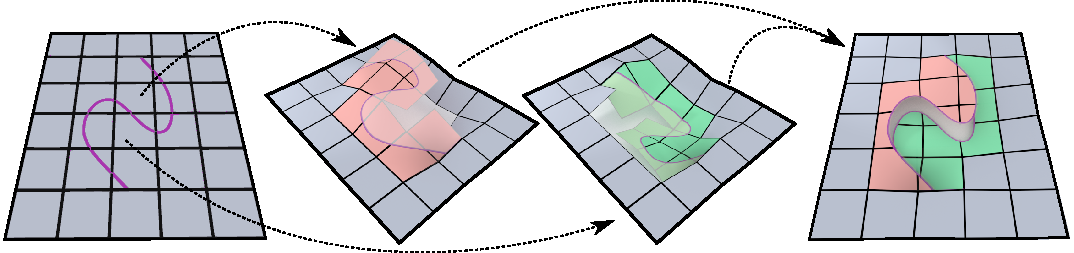
\includegraphics[width=.9\textwidth]{chapter_gridiron/images/New_HybridLattice2.pdf}
    % \includegraphics[width=.25\textwidth]{/tmp/foo.png}
    \vspace*{-.1in}
    \caption{Illustration of non-grid aligned topology change}{ A cutting path
    (far left) gives rise to new cells on either side of the cut
    (center), allowing the lattice to be divided below cell resolution
  (far right).}
    \vspace*{-.15in}
    \label{Fig:MaterialContinuityPreview}
  \end{figure}
  
  \section{Engineering A Solid Foundation}

  The following chapters will discuss in more detail some of the
  important engineering challenges and present techniques to overcome
  them. The primary goal is to demonstrate a set of related approaches
  that work well with each other and can be used to construct a highly
  performant, yet flexible foundation for a plastic surgery
  Simulation Assisted Visual System (SAVS). After a short related work section, highlighting some
  informative prior work, there will be several technical chapters
  dealing with the topics below. Finally, there will be a brief
  discussion section which will touch briefly on remaining
  philosophical issues and technical conclusions.

    \paragraph{Thin Feature Support}~ Due to the nature of the
      application, ensuring our simulated tissue can support thin
      geometric features, arising from incising tissue or simply the
      original tissue itself, is critical. What do we mean by support?
      In particular, our simulations need to be able to represent this
      geometry correctly within an embedded lattice deformer without
      compromising performance and accommodating behaviors like self
      collision. The current danger we face is that by embedding
      geometry in a lattice, instead of making our simulation elements
      conforming, we will not only loose accuracy around the boundary
      but potentially create unrealistic behavior by incorrectly connecting
      material across gaps unresolved by the lattice. In Chapters
      \ref{chp:nonmanifold} and \ref{chp:parallelization}, we'll look at
      solutions to these concerns via a process of non-manifold embedding.

    \paragraph{Optimized Lattice Deformers}~ We defined a
      SAVS to be an interactive system, and in order to use
      elastic simulation as a supporting technology we must ensure it
      can maintain sufficient levels of interactivity. Thus simulation
      performance is a key engineering challenge for us. Several times in this
      chapter we have mentioned that embedding lattice deformers were
      picked as the discretization model of choice over competing
      solutions, such as conforming mesh designs, due to their
      performance opportunities. These opportunities stem from their
      implicit data structures and regularity. These qualities reduce
      the amount of information than needs to read in order to access
      the store simulation data and allow for simplified computational
      designs.  However, these advantages do not come for free. In
      Chapters \ref{chp:parallelization} and \ref{chp:macroblocks}, we'll show
      how these properties can be exploited to create hardware aware
      algorithms for the solutions to the elasticity equations
      presented in this chapter. 
      
    \paragraph{Support for Non-linearity}~ While linear elastic
      materials are popular and easy to simulate, they fall short of
      the complexities observed in real biological material. While
      this document doesn't make any claim at delivering such
      materials, which require significant testing and validation
      against real tissue properties, we do wish to support these
      materials effectively. Moreover, even with relatively simple
      material models, adding additional constraints (either from
      user interactions or from contact) can make the problem
      non-linear. In Chapter \ref{chp:macroblocks}, we demonstrate a
      powerful generic technique for solving these highly non-linear
      problems, allowing for rapid convergence onto a correct
      solution.
      
    \paragraph{Deployment}~ While often overlooked, it is equally
      important to deliver a finished simulation to a user as it is to
      perform the simulation quickly and correctly. In Chapter
      \ref{chp:deployment}, we'll explore solutions for presenting
      simulated surgery operations to a multi-user environment. In
      particular, we'll look at issues such as available operating
      environments, suitability of cloud services, and maintainability.
   
  
  
%%% Local Variables:
%%% mode: latex
%%% TeX-master: "../document"
%%% End:
